\section{GPIO}
\emph{General Purpose Input/Output} (GPIO)

Input/output (I/O) is the interface between our digital microcontroller (MCU) and the rest of the world.
Each MCU has pins which its software uses to read input and write output.

Some pins are general purpose I/O, but some are used to power the MCU (VDD, GND) and some pins are
special (oscillator, clock pins), can to analog to digital I/O or vice versa, or more complex digital I/O (SPI, I2C, UART).

Digital input reads the pin to check if an external voltage is applied. Digital output drives the voltage on the pin. More advanced circuity performs
digital-to-analog conversion (DAC) or analog-to-digital (ADC).

The layout of every GPIO pin port looks like Figure \ref{fig:gpio}

\begin{figure}
    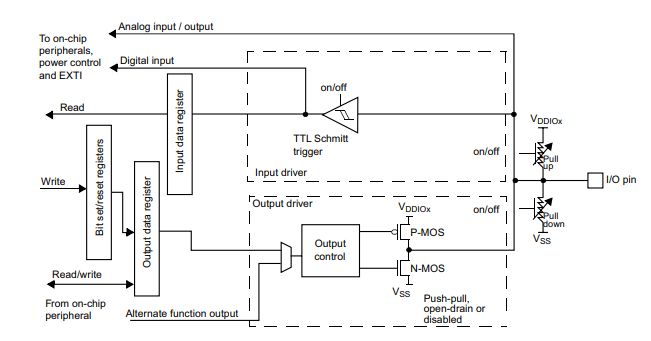
\includegraphics{images/gpio.png}
    \caption{GPIO Layout}
    \label{fig:gpio}
\end{figure}

Each MCU has multiple GPIO ports A, B, etc. Each port has multiple
GPIO bits (typically 8).

\subsection{Output}

The way output works is that an output bit is written
into the Output Data Register (ODR). Then the output driver
reads the ODR and drives the pin either high or low depending on
the value of the ODR bit. The voltage then appears on the I/O pin.

The GPIO can be configured as either read or write, output mode of push-pull
or open drain, output speed, and more.

In push-pull mode, we have need of a buffer to increase the output voltage
of the MCU so that when the output of the software is 1 the output
of the GPIO pin is VCC. This is accomplished with two NOT gates. If the software
write a 1, then the controller outputs a 0 to a NOT gate, which pulls the
output pin to 1. Basically, in push-pull mode the MCU actively drives the pin
low for 0 or high for 1.

In open drain mode, the MCU drives the output to low, but floats in 1. That is
the GPIO pin can be 0 volts, but it cannot be VCC. Basically, it can actively
drive a pin low for 0, but leaves the pin floating for 1. Open drain mode
is useful when there are multiple outputs. Two output pins can be tied together,
which isn't possible with push-pull outputs because one could be high and one low,
causing a short circuit. Thus, all tied pins must be open drain to avoid short circuits.
Any one of them can drive the shared output low, while a pull-up resistor passively
pulls the wire up to high when no MCU is driving it to low.
\marginnote{This is how I23 works. More details to follow in the unit of I2C.}

Another configurable is output speed, the speed of voltage rising and falling.
A faster GPIO is good for fast communication, but higher speed increases
electromagnetic interference and power consumption.

A related concept is slew rate, defined as
\begin{equation}
    \max(\frac{\Delta V}{\Delta t})
\end{equation}

\subsection{Input}

With input, an external circuit applies a voltage to the I/O pin.
The input driver converts the voltage to either 1 or 0. The input
is then sampled into the Input Data Register (IDR) every clock cycle.

In real life, the input voltage is noisy and messy. We add a Schmitt trigger
to smooth it, reduce noise, and increase the slew rate to make it suitable
for our digital circuit. Recall that a Schmitt trigger is just a buffer
that is immune to oscillating issues because it has a low and high threshold.
When the input signal crosses the high threshold, the output of the Schmitt
trigger is high. It stays high until the input signal crosses the low threshold,
at which point the output of the Schmitt trigger goes low.

Electricity in the real world is unfortunately messy.
Consider the circuit in Figure \ref{fig:led-circuit}.

\begin{figure}[h]
    \centering
    \begin{circuitikz}[american]
        % VDD power supply
        \draw (1.5,2.5) node[buffer] (mybuffer) {};
        \node at (0,4) {VDD};
        \draw (0,4) to[short] (0,3.5);

        % Switch
        \draw (0,3.5) to[nos] (0,2.5);
        \node at (-0.5,3) {};

        % Buffer (simple triangle)
        \draw (0,2.5) to[short] (1,2.5);
        \draw (2,2.5) to[short] (2.5,2.5);

        % Resistor
        \draw (2.5,2.5) to[R, l=$R$] (4,2.5);

        % LED
        \draw (4,2.5) to[led] (4,1);

        % Ground
        \draw (4,1) to[short] (4,0.5);
        \node[ground] at (4,0.5) {};
    \end{circuitikz}
    \caption{LED Control Circuit}
    \label{fig:led-circuit}
\end{figure}

You would expect that the circuit turns off when
the switch is open. However, the input to the buffer
would be floating, so the output of the buffer is unpredictable.